\documentclass[svgnames,11pt]{beamer}
\input{/home/tof/Documents/Cozy/latex-include/preambule_commun.tex}
\input{/home/tof/Documents/Cozy/latex-include/preambule_beamer.tex}
%\usepackage{pgfpages} \setbeameroption{show notes on second screen=left}
\author[]{Christophe Viroulaud}
\title{Construire un labyrinthe}
\date{\framebox{\textbf{Algo 23}}}
%\logo{}
\institute{Terminale - NSI}

\begin{document}
\begin{frame}
    \titlepage
\end{frame}
\section{Types de labyrinthe}
\begin{frame}
    \frametitle{Types de labyrinthe}

    \begin{center}
        \centering
        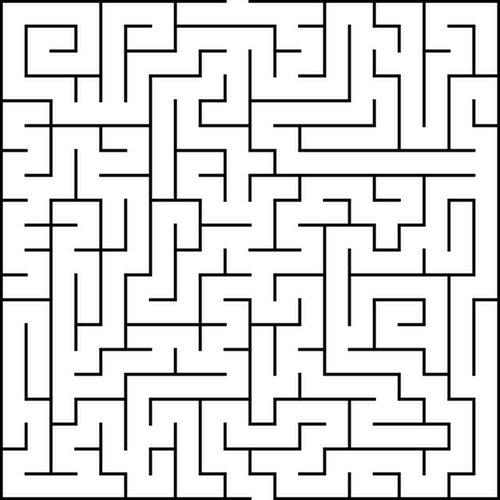
\includegraphics[width=6cm]{ressources/labyrinthe.png}
        \captionof{figure}{Un labyrinthe peut être représenté par un graphe.    }
    \end{center}
\end{frame}

\begin{frame}
    \frametitle{}

    \begin{aretenir}[Remarque]
        Il existe plusieurs catégories de labyrinthe. Considérons un labyrinthe où:
        \begin{itemize}
            \item tous les sommets sont atteignables,
            \item  on ne peut pas tourner en rond.

        \end{itemize}
    \end{aretenir}

\end{frame}
\begin{frame}
    \frametitle{}
    \begin{center}
        \centering
        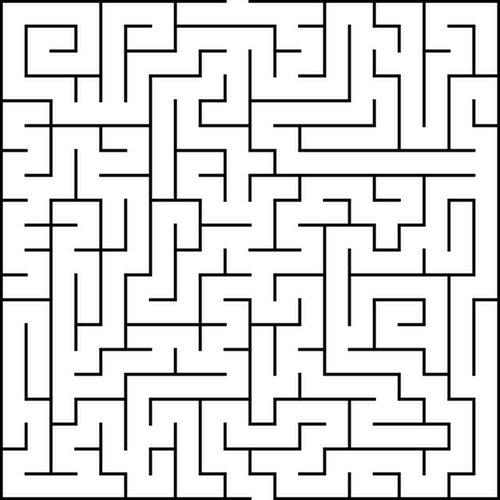
\includegraphics[width=6cm]{ressources/labyrinthe.png}
        \captionof{figure}{Un labyrinthe est un graphe non orienté et acyclique.}
    \end{center}


\end{frame}
\section{Construire un labyrinthe}
\begin{frame}
    \frametitle{Construire un labyrinthe}

    \begin{center}
        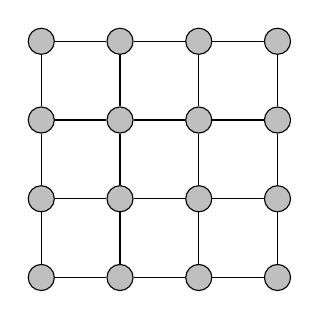
\begin{tikzpicture}
            \foreach \x in {0,1,...,3}
            {
                \node[draw,circle,fill=gray!50] (\x)at(0+\x,0) {};
                \node[draw,circle,fill=gray!50] (\x+1)at(0+\x,1) {};
                \node[draw,circle,fill=gray!50] (\x+2)at(0+\x,2) {};
                \node[draw,circle,fill=gray!50] (\x+3)at(0+\x,3) {};
                \draw (\x)--(\x+1);
                \draw (\x+2)--(\x+1);
                \draw (\x+2)--(\x+3);
            }
            \foreach \x/\y in {0/1,1/2,2/3}
            {
                \draw (\x)--(\y);
                \draw (\x+1)--(\y+1);
                \draw (\x+2)--(\y+2);
                \draw (\x+3)--(\y+3);
            }
        \end{tikzpicture}
        \captionof{figure}{Graphe de départ}
    \end{center}

\end{frame}
\begin{frame}
    \frametitle{}

    \begin{center}
        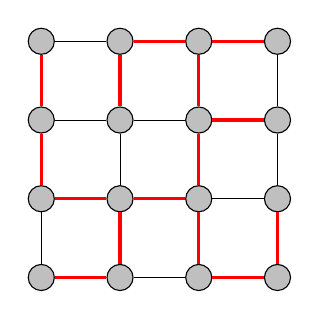
\begin{tikzpicture}
            \foreach \x in {0,1,...,3}
            {
                \node[draw,circle,fill=gray!50] (\x)at(0+\x,0) {};
                \node[draw,circle,fill=gray!50] (\x+1)at(0+\x,1) {};
                \node[draw,circle,fill=gray!50] (\x+2)at(0+\x,2) {};
                \node[draw,circle,fill=gray!50] (\x+3)at(0+\x,3) {};
                \draw[very thin] (\x)--(\x+1);
                \draw[very thin] (\x+2)--(\x+1);
                \draw[very thin] (\x+2)--(\x+3);
            }
            \foreach \x/\y in {0/1,1/2,2/3}
            {
                \draw[very thin] (\x)--(\y);
                \draw[very thin] (\x+1)--(\y+1);
                \draw[very thin] (\x+2)--(\y+2);
                \draw[very thin] (\x+3)--(\y+3);
            }
            \draw[red, very thick] (0)--(1);
            \draw[red, very thick] (1+1)--(1);
            \draw[red, very thick] (0+1)--(1+1);
            \draw[red, very thick] (1+1)--(2+1);
            \draw[red, very thick] (2+1)--(2);
            \draw[red, very thick] (2)--(3);
            \draw[red, very thick] (3+1)--(3);
            \draw[red, very thick] (2+2)--(2+1);
            \draw[red, very thick] (2+2)--(2+3);
            \draw[red, very thick] (2+2)--(2+1);
            \draw[red, very thick] (0+2)--(0+1);
            \draw[red, very thick] (0+2)--(0+3);
            \draw[red, very thick] (2+3)--(1+3);
            \draw[red, very thick] (1+3)--(1+2);
            \draw[red, very thick] (2+3)--(3+3);
            \draw[red, very thick] (2+2)--(3+2);

        \end{tikzpicture}
        \captionof{figure}{\centering En effectuant un parcours en profondeur, on peut construire un labyrinthe.}
    \end{center}
\note{Il n'y a pas de cycle.}
\end{frame}
\section{Utiliser une bibliothèque graphique}
\begin{frame}
    \frametitle{Utiliser une bibliothèque graphique}

    \begin{aretenir}[]
    La bibliothèque \textbf{\texttt{tkinter}} est intégrée dans l'interpréteur Python. Elle permet de créer un affichage graphique.
    \end{aretenir}

\end{frame}
\begin{frame}[fragile]
    \frametitle{}

\begin{center}
\begin{lstlisting}[language=Python , basicstyle=\ttfamily\small, xleftmargin=2em, xrightmargin=2em]
import tkinter

TAILLE = 5
DIM = 50

fenetre = tkinter.Tk()
fenetre.title("Dessiner")
canevas = tkinter.Canvas(fenetre,
                         width=DIM * TAILLE,
                         height=DIM * TAILLE,
                         bg="#FFFFFF")
canevas.pack()
\end{lstlisting}
\captionof{code}{\centering Créer une fenêtre \textbf{\texttt{tkinter}} et un canevas.}
\label{CODE}
\end{center}

\end{frame}
\begin{frame}[fragile]
    \frametitle{}

\begin{center}
\begin{lstlisting}[language=Python , basicstyle=\ttfamily\small, xleftmargin=2em, xrightmargin=1em]
canevas.create_line(0, 0, 10, 10, fill="black", width=2)
\end{lstlisting}
\captionof{code}{Tracer une ligne de (0,0) à (10,10)}
\label{CODE}
\end{center}
\begin{activite}
\begin{enumerate}
    \item Créer une grille de \textbf{\texttt{TAILLE}} lignes et \textbf{\texttt{TAILLE}} colonne.
    \item Placer la ligne suivante en fin de programme:
    \begin{lstlisting}[language=Python , basicstyle=\ttfamily\small, xleftmargin=2em, xrightmargin=2em]
fenetre.mainloop()
\end{lstlisting}
\end{enumerate}
\end{activite}
\end{frame}
\begin{frame}[fragile]
    \frametitle{Correction}

\begin{center}
\begin{lstlisting}[language=Python , basicstyle=\ttfamily\small, xleftmargin=0.2em, xrightmargin=0em]
for i in range(TAILLE):
    canevas.create_line(i*DIM, 0, 
                        i*DIM, TAILLE*DIM, 
                        fill="black", width=2)
    canevas.create_line(0, i*DIM, 
                        TAILLE*DIM, i*DIM,  
                        fill="black", width=2)
\end{lstlisting}
\end{center} 
\end{frame}
\begin{frame}
    \frametitle{}
\begin{activite}
\begin{enumerate}
    \item Télécharger et extraire le dossier compressé \textbf{\texttt{labyrinthe-annexe.zip}} sur le site \url{https://cviroulaud.github.io}
    \item Analyser le code. Comprendre le mécanisme pour diriger le cercle bleu.
\end{enumerate}
\end{activite}
\end{frame}
\end{document}